\documentclass{beamer}
\usetheme{Madrid}

\usepackage{cmap}
\usepackage[T2A]{fontenc}
\usepackage[russian,english]{babel}
\usepackage[utf8]{inputenc}
\usepackage{amsmath, amssymb}
\usepackage{minted}
\usepackage{hologo}

\usepackage{algorithm2e}
\usepackage{algorithmic}
\usepackage{float}

% \newtcbox{\mybox}{blank, on line, opacitytext=0.5}

\title[Ускорение обучения языковых моделей]{Методы предобработки текстовых данных для ускорения обучения языковых моделей}

\author[Сурков М.К.]{Сурков Максим Константинович\\
 	{\footnotesize Научный руководитель: Ямщиков Иван Павлович}
}
\institute[НИУ ВШЭ СПБ]{Санкт-Петербургская школа физико-математических и компьютерных наук \\ НИУ ВШЭ СПБ}
\date{17 марта 2021 г.}

\begin{document}

\frame{\titlepage}

\begin{frame}
\frametitle{Обработка естественного языка в реальной жизни}
\begin{columns}
	\column{0.5\textwidth}
	\begin{itemize}
		\item социальные сети
		\item электронная почта
		\item службы доставки
		\item голосовые помощники
		\item переводчики
		\item чат боты
	\end{itemize}
	\column{0.5\textwidth}
	
\includegraphics[scale=0.2]{nlp_real_life.png}
\end{columns}
\end{frame}

\begin{frame}
\frametitle{Задачи обработки естественного языка}
\begin{enumerate}
	\item классификация последовательностей
		\begin{itemize}
			\item спам
			\item грубая речь\footnote[1]{G. H. Paetzold et al., SemEval'19 Task 5: Hate Speech Identification with RNN.}
		\end{itemize}
	\item генерация выходной последовательности из исходной
		\begin{itemize}
			\item машинный перевод
			\item ответы на вопросы
		\end{itemize}
	\item выделение информации из последовательностей
		\begin{itemize}
			\item выделение именованных сущностей\footnote[2]{Vikas Yadav et al., SemEval'19 Task 12: Deep-Affix Named Entity Recognition of Geolocation Entities. ACL'19}
		\end{itemize}
\end{enumerate}

\end{frame}

\begin{frame}
	\frametitle{Современные методы решения задач обработки естественного языка}
	\begin{enumerate}
		\item Механизм внимания\footnote[1]{Ashish Vaswani et al., Attention Is All You Need, 2017}
		\item {\bf BERT} (Google)\footnote[2]{Jacob Devlin et al., BERT: Pre-training of Deep Bidirectional Transformers for Language Understanding, 2019}
		\item GPT-3 (OpenAI)\footnote[3]{Tom B. Brown et al., Language Models are Few-Shot Learners, 2020}
	\end{enumerate}
\end{frame}

\begin{frame}
	\frametitle{BERT. Использование}
	\begin{center}
		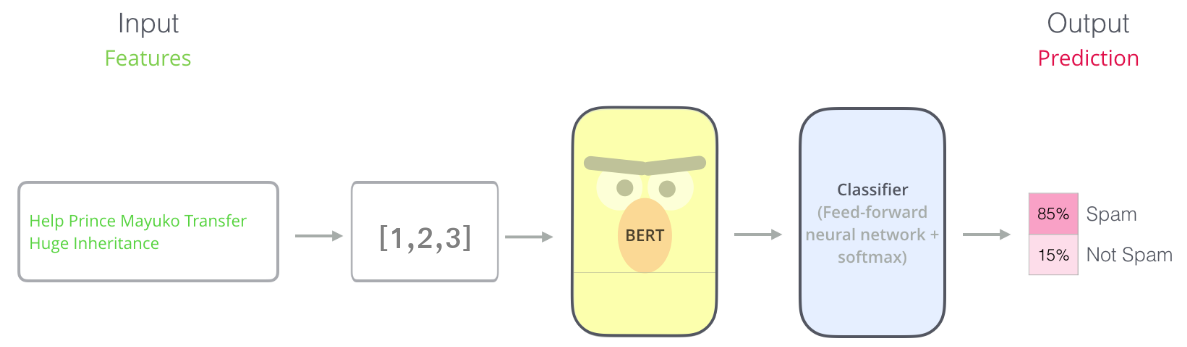
\includegraphics[scale=0.35]{bert_usage.png}
	\end{center}
\end{frame}

\begin{frame}
	\frametitle{BERT. Обучение}
	\begin{center}
		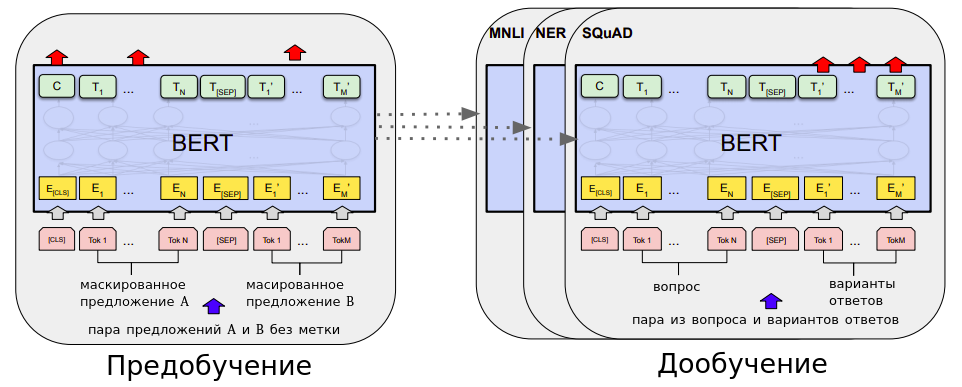
\includegraphics[scale=0.35]{bert_train.png}
	\end{center}
\end{frame}

\begin{frame}
	\frametitle{BERT. Требуемые ресурсы}
	\begin{itemize}
		\item количество параметров: $110M - 340M$
		\item время на предобучение: от 2-4 дней до 1-2 недель\footnote[1]{При использовании 1x-4x GPU Nvidia Tesla V100 32Gb}
		\begin{itemize}
			\item мировой рекорд: 47 минут на {\bf 1472} V100 GPU\footnote[2]{https://developer.nvidia.com/blog/training-bert-with-gpus}
		\end{itemize}
		\item время на дообучение: 1-2 дня
		\item размеры данных:
			\begin{table}
				\begin{tabular}{l|c}
					Датасет & Размер \\
					\hline\hline
					Wikipedia & 3-600M \\
					HND & 600k-2M \\
					s140 & 1.6M \\
					IWSLT & 200-230k \\
					QQP & 364k \\
					MNLI & 393k \\
				\end{tabular}
			\end{table}
	\end{itemize}
\end{frame}

\begin{frame}
	\frametitle{BERT. Существующие методы оптимизации}
	\begin{itemize}
		\item квантизация\footnote[1]{Sheng Shen et al., Q-BERT: Hessian Based Ultra Low Precision Quantization of BERT, 2019}
		\item дистилляция\footnote[2]{Victor Sanh et al., DistilBERT, a distilled version of BERT: smaller, faster, cheaper and lighter, 2020}
		\item прунинг\footnote[3]{Hassan Sajjad et al., Poor Man’s BERT: Smaller and Faster Transformer Models, 2020}
	\end{itemize}
\end{frame}

\begin{frame}
	\frametitle{Обучение с расписанием. Начало}
	
	\begin{center}
		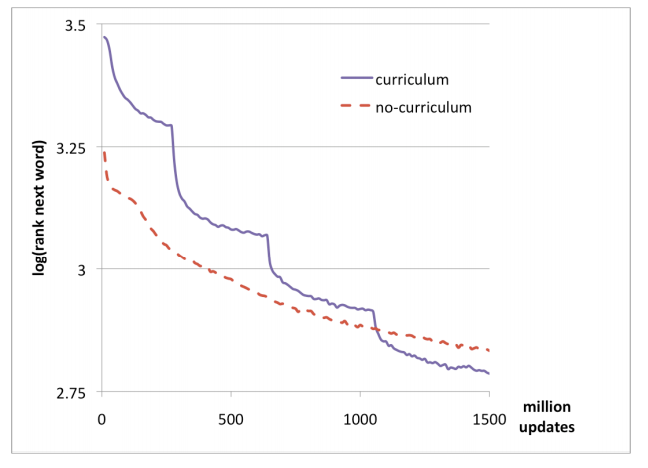
\includegraphics[scale=0.4]{bengio_exp1}
	\end{center}
	
	\let\thefootnote\relax\footnotetext{Y. Bengio et al., Curriculum learning, 2009}
\end{frame}

\begin{frame}
	\frametitle{Обучение с расписанием. Применение}
	\begin{itemize}
		\item компьютерное зрение\footnote[1]{Guy Hacohen, Daphna Weinshall, On The Power of Curriculum Learning in Training Deep Networks, 2019}

		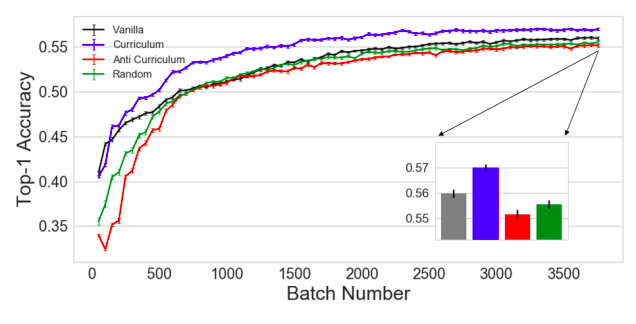
\includegraphics[scale=0.3]{curriculum_learning_cv}
		
		\item обучение с подкреплением\footnote[2]{Sanmit Narvekar et al., Curriculum Learning for Reinforcement Learning Domains: A Framework and Survey, 2020}
		
		\item глубокое обучение\footnote[3]{Mermer et al., Scalable Curriculum Learning for Artificial Neural Networks, 2017}
	\end{itemize}
\end{frame}

\begin{frame}
	\frametitle{Обучение с расписанием в обработке языка}		\let\thefootnote\relax\footnotetext{E. A. Platanios et al., Competence-based Curriculum Learning for Neural Machine Translation, ACL'19}
	\begin{itemize}
		\item Задача: машинный первод
		\item Модель: BERT, LSTM
		\item Датасеты: IWSLT'15, IWSLT'16, WMT'16
		\item Алгоритм:
			\begin{columns}
				\column{0.5\textwidth}
					\begin{enumerate}
						\item сортируем тексты по сложности (длина, логарифм веротности правдоподобия)
						\item в течение $T$ шагов (рассмотрим шаг $t$)
						\begin{itemize}
							\item считаем $c(t) \in [0, 1]$
							\item строим батч из $c(t)$ {\bf первых} текстов корпуса
							\item шаг обучения
						\end{itemize}
					\end{enumerate}
				\column{0.5\textwidth}
				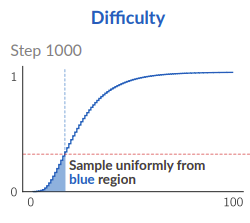
\includegraphics[scale=0.6]{acl19_algo.png}
			\end{columns}
	\end{itemize}
\end{frame}

\begin{frame}
	\frametitle{Обучение с расписанием в обработке языка}
	\begin{center}
		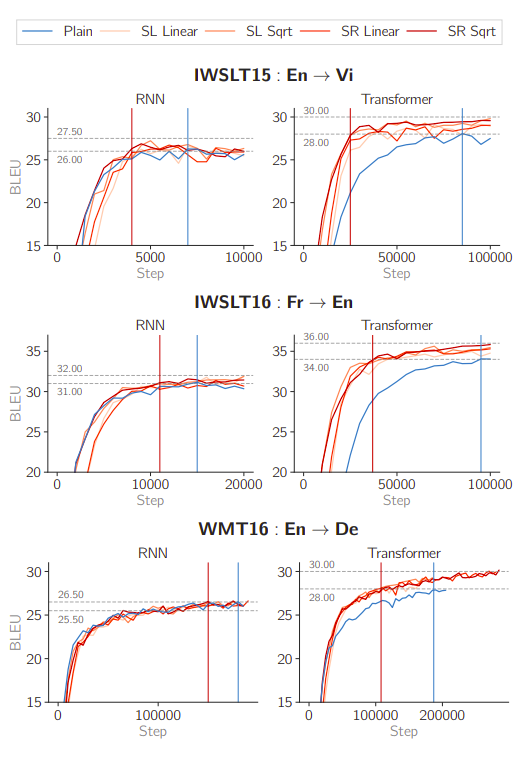
\includegraphics[scale=0.3]{acl19_results}
	\end{center}
\end{frame}

\begin{frame}
	\frametitle{Обучение с расписанием в обработке языка}		\let\thefootnote\relax\footnotetext{Benfeng Xu et al., Curriculum Learning for Natural Language Understanding, ACL'20}
\end{frame}

\begin{frame}
	\frametitle{Обучение с расписанием в обработке языка. Направления для исследований}
\end{frame}


\end{document}